../cictikz/src/cictikz/data/tex/cictikz_preamble.tex

% GR07's measured noise against f, the fractional part of its
% period measured in 64 MHz clock cycles. The output alternates between N
% and N+1 whole cycles, and to average out at N+f a fraction f of the
% periods must come out long - a Bernoulli process, whose spread goes as
% the square root of f(1-f). The dashed curve is that shape with a single
% scale factor fitted; it follows the measurements with r = 0.997. The
% noise is smallest where the period is nearly a whole number of cycles,
% because there is then almost nothing for the quantiser to dither
% about.
%
% Generated by py/tikzplot.py. Edit the script in ex/ that
% produced it and re-run that, not this file.

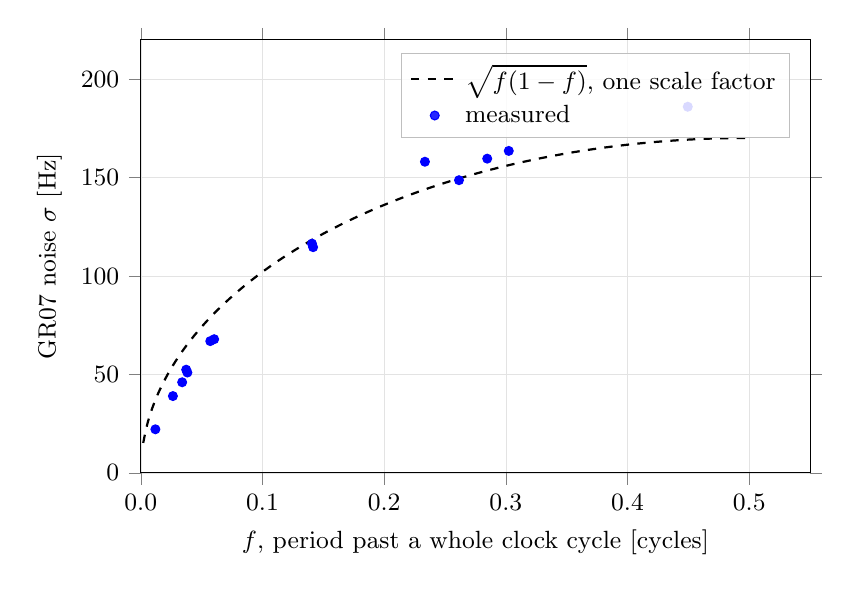
\begin{tikzpicture}[thick]

\begin{axis}[
  width=8.5cm,
  height=5.5cm,
  scale only axis,
  grid=both,
  grid style={gray!22, very thin},
  tick align=outside,
  tick label style={font=\small},
  label style={font=\small},
  title style={font=\small, yshift=-1mm},
  legend cell align=left,
  legend style={font=\small, draw=gray!50, fill=white, fill opacity=0.85, text opacity=1},
  xlabel={$f$, period past a whole clock cycle [cycles]},
  ylabel={GR07 noise $\sigma$ [Hz]},
  scaled x ticks=false,
  xticklabel style={/pgf/number format/fixed, /pgf/number format/zerofill, /pgf/number format/precision=1},
  xmin=0,
  xmax=0.55,
  ymin=0,
  ymax=220,
  legend pos=north east
]
\addplot[black, thick, dashed, mark=none] coordinates {(0.002,15.201) (0.004,21.476) (0.006,26.276) (0.008,30.311) (0.01,33.854) (0.012,37.048) (0.014,39.976) (0.016,42.693) (0.018,45.236) (0.02,47.635) (0.022,49.909) (0.024,52.075) (0.026,54.145) (0.028,56.132) (0.03,58.042) (0.032,59.884) (0.034,61.663) (0.036,63.385) (0.038,65.054) (0.04,66.675) (0.042,68.25) (0.044,69.783) (0.046,71.277) (0.048,72.734) (0.05,74.155) (0.052,75.544) (0.054,76.902) (0.056,78.23) (0.058,79.531) (0.06,80.804) (0.062,82.053) (0.064,83.277) (0.066,84.478) (0.068,85.656) (0.07,86.813) (0.072,87.95) (0.074,89.067) (0.076,90.165) (0.078,91.245) (0.08,92.307) (0.082,93.352) (0.084,94.381) (0.086,95.393) (0.088,96.391) (0.09,97.373) (0.092,98.341) (0.094,99.294) (0.096,100.23) (0.098,101.16) (0.1,102.07) (0.102,102.98) (0.104,103.86) (0.106,104.74) (0.108,105.61) (0.11,106.46) (0.112,107.3) (0.114,108.13) (0.116,108.96) (0.118,109.77) (0.12,110.57) (0.122,111.36) (0.124,112.14) (0.126,112.91) (0.128,113.67) (0.13,114.43) (0.132,115.17) (0.134,115.91) (0.136,116.63) (0.138,117.35) (0.14,118.06) (0.142,118.76) (0.144,119.46) (0.146,120.14) (0.148,120.82) (0.15,121.49) (0.152,122.16) (0.154,122.81) (0.156,123.46) (0.158,124.1) (0.16,124.74) (0.162,125.36) (0.164,125.99) (0.166,126.6) (0.168,127.21) (0.17,127.81) (0.172,128.4) (0.174,128.99) (0.176,129.57) (0.178,130.15) (0.18,130.72) (0.182,131.28) (0.184,131.84) (0.186,132.39) (0.188,132.94) (0.19,133.48) (0.192,134.01) (0.194,134.54) (0.196,135.07) (0.198,135.59) (0.2,136.1) (0.202,136.61) (0.204,137.11) (0.206,137.61) (0.208,138.1) (0.21,138.59) (0.212,139.07) (0.214,139.54) (0.216,140.02) (0.218,140.48) (0.22,140.95) (0.222,141.4) (0.224,141.86) (0.226,142.31) (0.228,142.75) (0.23,143.19) (0.232,143.62) (0.234,144.05) (0.236,144.48) (0.238,144.9) (0.24,145.31) (0.242,145.73) (0.244,146.13) (0.246,146.54) (0.248,146.94) (0.25,147.33) (0.252,147.72) (0.254,148.11) (0.256,148.49) (0.258,148.87) (0.26,149.24) (0.262,149.61) (0.264,149.98) (0.266,150.34) (0.268,150.7) (0.27,151.06) (0.272,151.41) (0.274,151.75) (0.276,152.1) (0.278,152.44) (0.28,152.77) (0.282,153.1) (0.284,153.43) (0.286,153.75) (0.288,154.07) (0.29,154.39) (0.292,154.7) (0.294,155.01) (0.296,155.32) (0.298,155.62) (0.3,155.92) (0.302,156.22) (0.304,156.51) (0.306,156.8) (0.308,157.08) (0.31,157.36) (0.312,157.64) (0.314,157.91) (0.316,158.19) (0.318,158.45) (0.32,158.72) (0.322,158.98) (0.324,159.24) (0.326,159.49) (0.328,159.74) (0.33,159.99) (0.332,160.23) (0.334,160.47) (0.336,160.71) (0.338,160.95) (0.34,161.18) (0.342,161.41) (0.344,161.63) (0.346,161.85) (0.348,162.07) (0.35,162.29) (0.352,162.5) (0.354,162.71) (0.356,162.92) (0.358,163.12) (0.36,163.32) (0.362,163.52) (0.364,163.71) (0.366,163.9) (0.368,164.09) (0.37,164.27) (0.372,164.46) (0.374,164.63) (0.376,164.81) (0.378,164.98) (0.38,165.15) (0.382,165.32) (0.384,165.48) (0.386,165.64) (0.388,165.8) (0.39,165.96) (0.392,166.11) (0.394,166.26) (0.396,166.4) (0.398,166.55) (0.4,166.69) (0.402,166.82) (0.404,166.96) (0.406,167.09) (0.408,167.22) (0.41,167.35) (0.412,167.47) (0.414,167.59) (0.416,167.71) (0.418,167.82) (0.42,167.93) (0.422,168.04) (0.424,168.15) (0.426,168.25) (0.428,168.35) (0.43,168.45) (0.432,168.54) (0.434,168.64) (0.436,168.72) (0.438,168.81) (0.44,168.89) (0.442,168.98) (0.444,169.05) (0.446,169.13) (0.448,169.2) (0.45,169.27) (0.452,169.34) (0.454,169.4) (0.456,169.46) (0.458,169.52) (0.46,169.58) (0.462,169.63) (0.464,169.68) (0.466,169.73) (0.468,169.78) (0.47,169.82) (0.472,169.86) (0.474,169.89) (0.476,169.93) (0.478,169.96) (0.48,169.99) (0.482,170.01) (0.484,170.04) (0.486,170.06) (0.488,170.08) (0.49,170.09) (0.492,170.1) (0.494,170.11) (0.496,170.12) (0.498,170.12) (0.5,170.12)};
\addlegendentry{$\sqrt{f(1-f)}$, one scale factor}
\addplot[blue, only marks, mark=*, mark size=1.6pt, mark=none] coordinates {(0.2847,159.6) (0.012,22.12) (0.0373,52.392) (0.2335,158.03) (0.4495,185.96) (0.1407,116.43) (0.0603,67.883) (0.034,46.007) (0.0264,38.993) (0.0383,50.952) (0.0571,66.906) (0.1416,114.64) (0.3024,163.54) (0.2615,148.66)};
\addlegendentry{measured}
\end{axis}

\end{tikzpicture}
\end{document}
